\documentclass{scrartcl}
\usepackage{base}


\author{Stefan Heid}
\title{Introduction to JPEG}
\begin{document}
\selectlanguage{english}
\maketitle
\tableofcontents
\newpage

\section{JPEG}
JPEG mainly relies on Transformation of the picture data to other domains. This is used to reduce Details from the image without loosing much perceptual Quality. This is possible because real Photographs usually have highly correlated pixels, which means, that neighbour pixels have most likely nearly the same or even the same Value.

JPEG also works, because Humans hardly recognize small changes in color. Therefore it is possible to obtain high compression ratios while preserving a quiet high image Quality.

\subsection{Algorithm}
\begin{enumerate}
\item Convertion of Color scheme
\item Splitting the Picture into Blocks
\item Discrete Cosine transform
\item Quantization
\item Entropy Coding of DC and AC coefficients
\end{enumerate}

\subsection{Converting Color Format}
Like in Digital and Analog Television JPEG starts with conversion the Color Scheme from RGB to $ YC_BC_R $ in order to reduce the resolution of color. This can be done, because changes in Lightness ar much more perceptual than changes in Color.

\subsection{Splitting the Picture in Blocks}
In the JPEG Algorithm the Picture will be cut into Blocks with 8x8 Pixels. Those Blocks will be processed separately. Even though the Compression could possibly be better when using the Algorithm on the whole picture than on blocks, it is not been done for two main reasons.
\begin{enumerate}
\item When removing Detail of the picture using the DCT and Quantization process, Jpeg relies on the fact that nearby pixels are correlated. When using this methodes on the whole picture, this correlation is of course not longer the case.
\item The DCT has a non linear calculation time complexity. The best implementations have a complexity of $ \mathcal{O}(n \log_2 n) $ which means, that doubling the Number of pixels of a Block results in more than more than doubling the calculation Time. In Fact, when one considers real Photographs with a couple of Million pixels this Property can cause serious performance Problems.
\end{enumerate}

\subsection{Discrete Cosine Transform}
The Discrete Cosine Transform or DCT convertes the 64 Pixels of the Block in that way that the Pixels rather show differences than concrete values. The First Value is Called DC coefficient which is something like the Average of the whole Block. The other coefficients, the so called AC, have quiet small value because of the assumed small amount of differences in one block. At this Stage of the algorithms (considering that the color Components $ C_B $ and $ C_R $ have not been down sampled) no compression has been done and all processes are reversible, but the Data is prepared to make this possible.

\subsection{Quantization}
In this part each pixel from the of the converted block will be divided by a value set a Matrix. The default Matrix is different for Chroma components and the Lighting component of the picture. Because this is the only lossy part, this is where the Quality variable comes into play. This Variable scales the values of the Quantization matrix. A higher Quality results in smaller values of the matrix and therefore less loss when rounding the values.

\begin{figure}
\centering
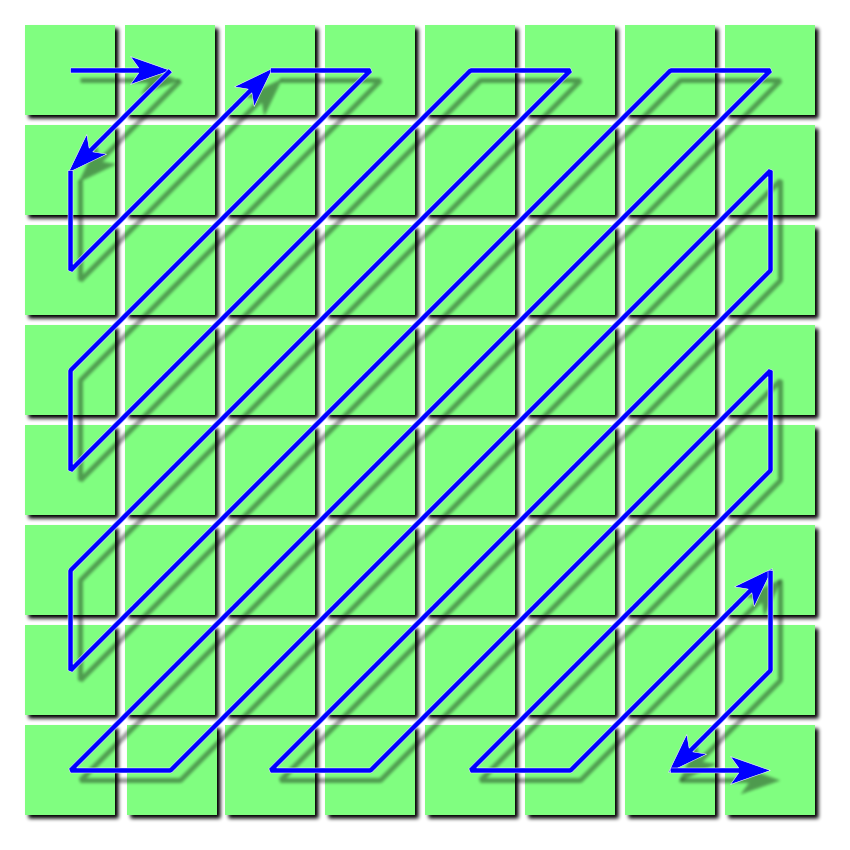
\includegraphics[width=0.5\linewidth]{./JPEG_ZigZag}
\caption{Zigzag Traverse through the Block}
\label{fig:JPEG_ZigZag}
\end{figure}

After division, the values are rounded, which leads to data loss. For the next processing Steps the Matrix Values will be traversed using a ZigZag pattern (see Figure \ref{fig:JPEG_ZigZag}). This is done because the left lower Corner of the matrix will have the smallest Values, because of the assumptions mentioned in the chapter above. The now linear array will have probably a lot of zeroes at the end which can be expressed using Runlength encoding.

\subsection{Huffman Coding}
After quantizing the matrices we will use four times Huffman encoding to encode our data. First i will introduce the Huffman encoding algorithm and later i will explain how it is used in JPEG.

In general Huffman encoding produces prefix free codes for a set of words to be encoded. Each of those words have a frequency, meaning a number of appearances in the matrixes of the Picture. Prefix free means, the codes can have different length, but when all codes are concatenated in a bit string it is always clear where one codeword ends and where the next one starts. This is of course important when decoding the huffman code.

The Huffman Algorithm uses a binary tree to create the codes. At first, all words are sorted accouring their frequency. In the next steps of the Algorithm, this frequency is used as a weight. The algorithm starts by taking the 2 nodes or words, with the minimum weight, and connecting them to a tree. His weight is the sum of the two nodes and he will be put back to the pool of available nodes. This goes on so long until there is just one more node/tree left. We have now a binary tree whose leaves are the words we wanted to encode.

Now we label each left edge with zero and each right edge with one. When we now traverse the tree from the root to each leave, we can read the code for every word.

In Jpeg the Huffman coding is done separately for the Chroma and the Lighting Values and there once for the DC coefficients and for the AC coefficients. This is done, because Huffman coding is then very efficient, when there are some words very frequent and and just a view rare. Because DC efficients are usually a lot higher than AC coefficents this division is very important.

The Entropy coding is also lossless and one of the most important parts of the Jpeg Algorithm. The Specification requires Huffman codes to be at maximum 16 bits. This can be achieved by rearranging parts of the tree in order to reduce its depth.

\subsection{Decompression}
Decompression uses basically the reverse Process. First step is a Entropy decoding using the Huffman Tables. Than we multiply the derived Data with the Quantization Tables. After the Inverse Cosine Transform the $ Yc_BC_R $ model is converted to RGB and so the original is restored, of course with some compression artifacts.

\subsection{Bitstream}


\section{JPEG2000}

\end{document}